\section{Problem Statement: Bipedal Walker Robot Control}
\label{sec:problem_statement}

\subsection{OpenAI Gym and Bipedal Walker Environment}
\label{ssec:gym_bipedal}

OpenAI Gym \cite{brockman_openai_2016} is an open source framework, 
containing many environments to service the development of 
reinforcement learning algorithms. 

\textit{BipedalWalker} environments~\cite{noauthor_bipedalwalker-v2_2021, noauthor_bipedalwalkerhardcore-v2_2021} are parts of Gym environment library. 
One of them is classical where the terrain is relatively smooth, while other is a hardcore version containing ladders, stumps and pitfalls in terrain. 
However, terrain is randomly generated at the beginning of each episode.
Those environments have continuous action and observation space. 
For both settings, the task is to move the robot forward as much as possible. 
Snapshots for both environments are depicted in \figref{fig:bipedal_walkers}.
\begin{figure}
	\begin{subfigure}{.5\textwidth}
		\centering
		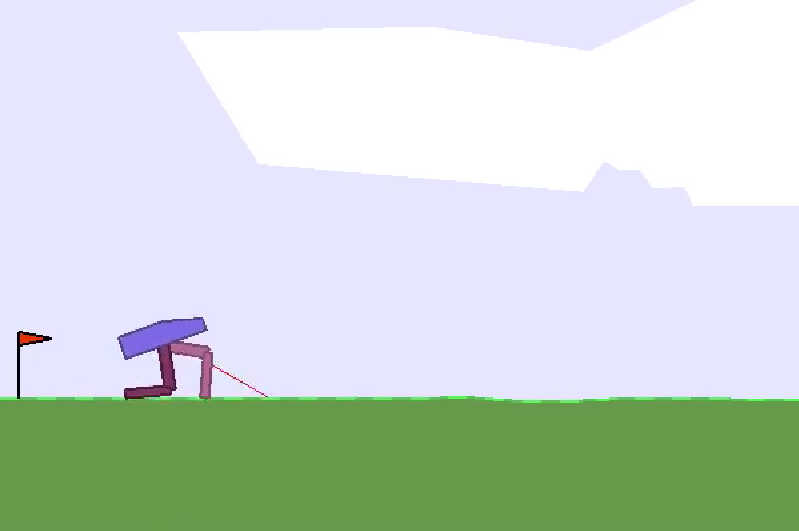
\includegraphics[width=0.9\linewidth]{figures/bipedal/classic.png}
		\caption{BipedalWalker-v3 Snapshot~\cite{noauthor_bipedalwalker-v2_2021}}
		\label{fig:bipedal_walker_classic}
	\end{subfigure}
	\begin{subfigure}{.5\textwidth}
		\centering
		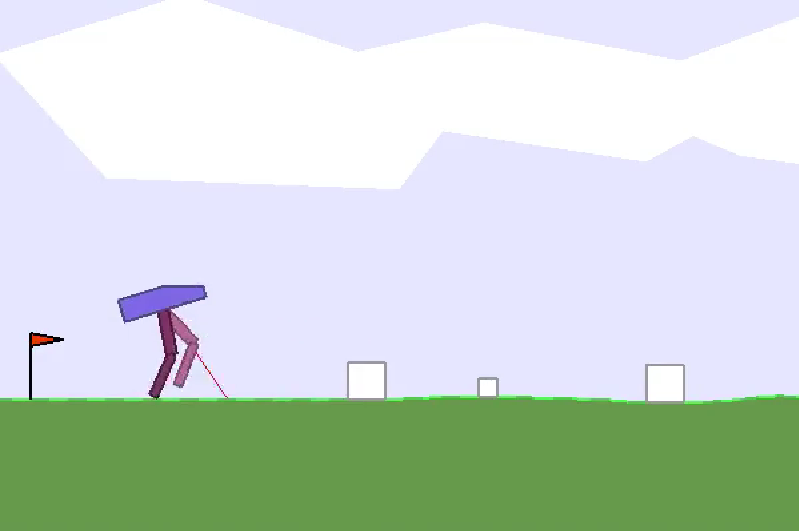
\includegraphics[width=0.9\linewidth]{figures/bipedal/hardcore.png}
		\caption{BipedalWalkerHardcore-v3 Snapshot~\cite{noauthor_bipedalwalkerhardcore-v2_2021}}
		\label{fig:bipedal_walker_hardcore}
	\end{subfigure}
	\caption{Bipedal Walkers Snapshots}
	\label{fig:bipedal_walkers}
\end{figure}

Locomotion of the Bipedal Walker is a difficult control problem due to following reasons: 
\begin{description}
	\item[Nonlinearity]. The dynamics are nonlinear, unstable and multimodal. 
	Dynamical behavior of robot changes for different situations 
	like ground contact, single leg contact and double leg contact.
	\item[Uncertainity]. The terrain where the robot walks may vary. 
	Designing a controller for all types of terrain is difficult.
	\item[Reward Sparsity]. Overcoming some obstacles requires a specific maneuver, which is hard to explore sometimes.	
	\item[Partially Observability]. The robot observes 
	ahead of it with lidar measurements and cannot observe behind. 
	In addition, it lacks of acceleration sensors.
\end{description}

These reasons make it hard to implement analytical methods for control tasks. 
However, approach can easily overcome nonlinearity and uncertainity problems.

On the other hand, reward sparsity problem brings local minimums to objective function of optimal control. It can be solved by a good exploration strategy and reward shaping. 

For the partial observability problem, more elegant solution is required. 
This is achieved by creating a belief state from the past observations to inform the agent. 
Agent uses this belief state to choose how to act. 
If belief state is evaluated sufficiently, 
this increases performance of the agent.
However, relying on observations is also possible, 
and this may be enough sometimes if advanced type of control is not required. 

\subsection{Deep Learning Library: PyTorch}
\label{dl_pytorch}
PyTorch is an open source library developed by Facebook's AI Research Lab (FAIR)~\cite{paszke_pytorch_2019}. 
It is based on Torch library~\cite{collobert_torch7_2011} and has Python and C++ interface. 
It is an automatic differentation library with accelerated mathematical operations backed by graphical processing units (GPUs). 
The clean pythonic syntax made it most famous deep learning tool among researches. 
